% ---
% Capa
% ---
\imprimircapa
% ---

% ---
% Folha de rosto
% (o * indica que haverá a ficha bibliográfica)
% ---
\imprimirfolhaderosto*
% ---

% ---
% Inserir a ficha bibliografica
% ---
% http://ficha.bu.ufsc.br/
\begin{fichacatalografica}
	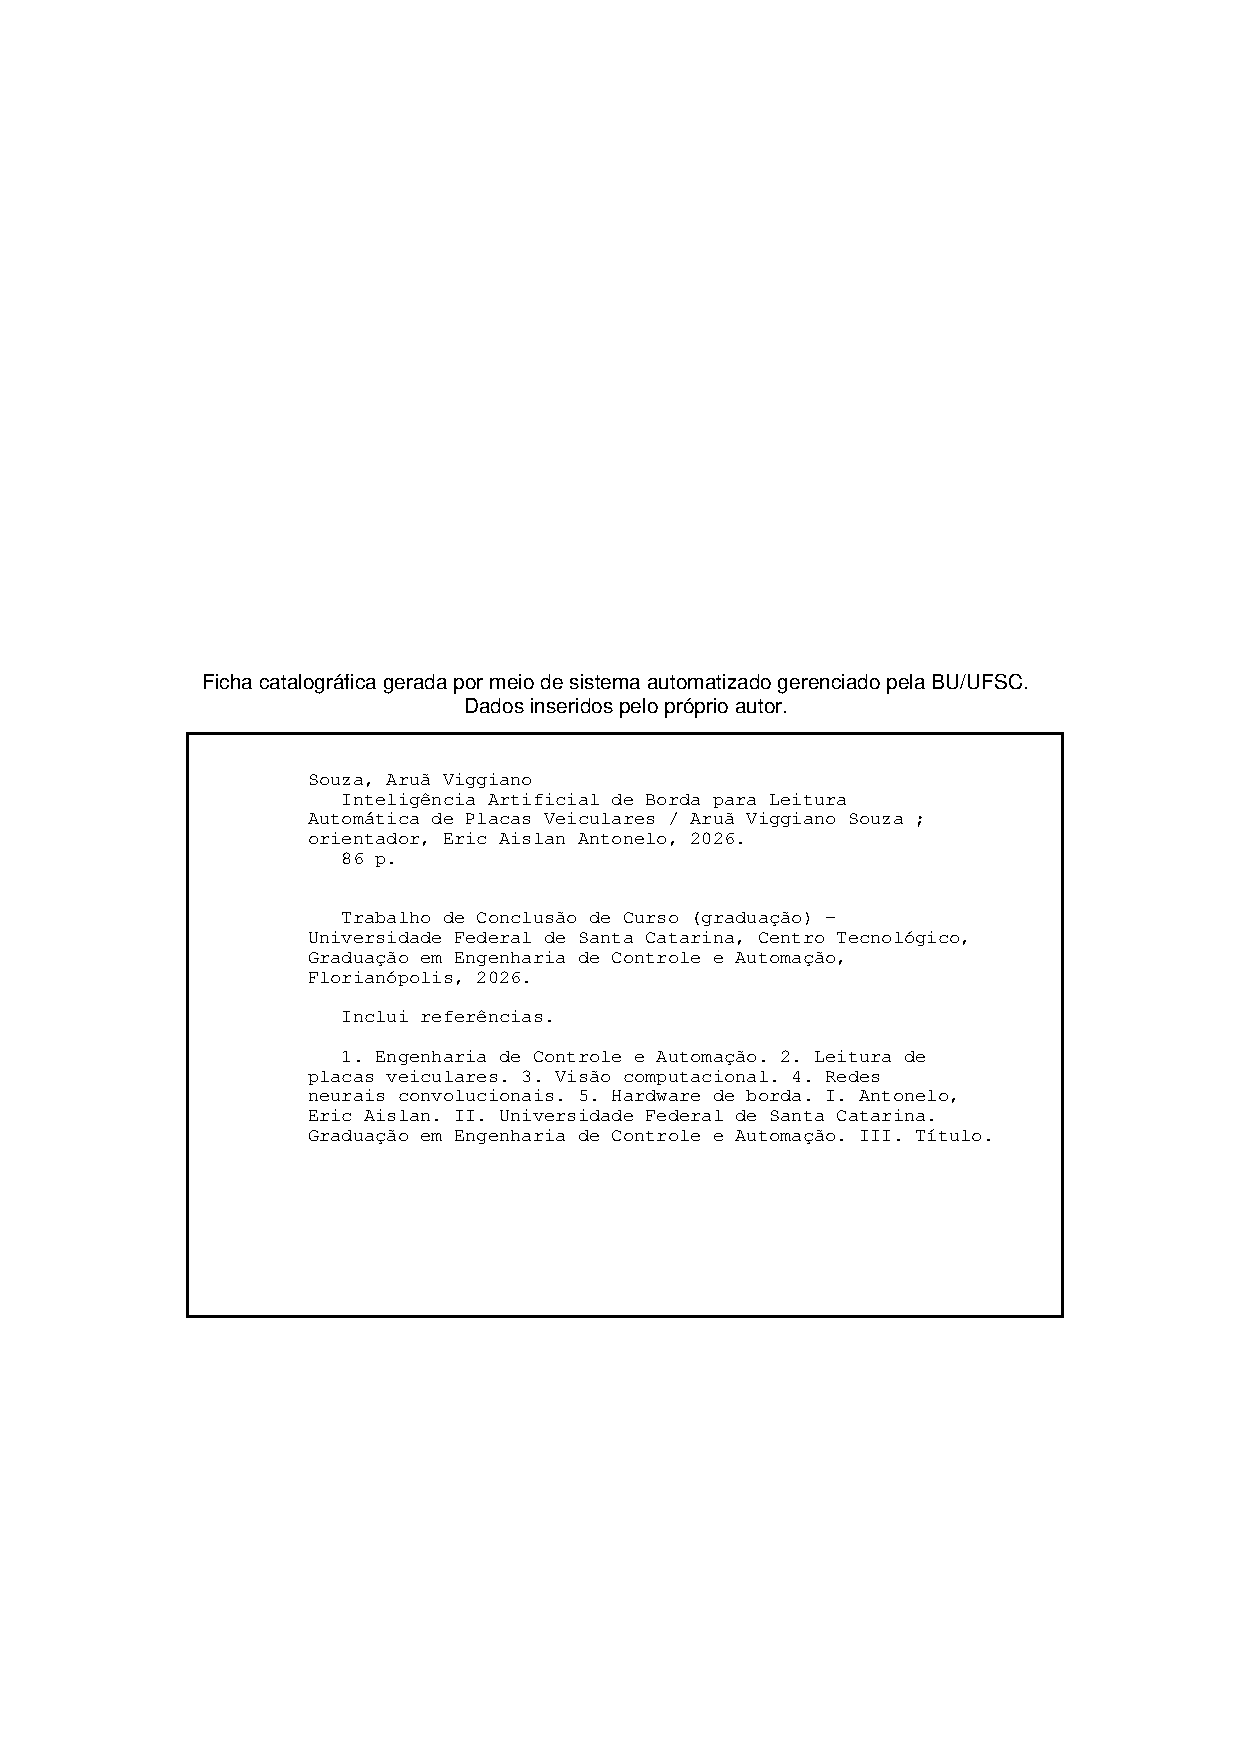
\includepdf{beforetext/Ficha_Catalografica.pdf}
\end{fichacatalografica}
% ---

% ---
% Inserir folha de aprovação
% ---
\begin{folhadeaprovacao}
	\OnehalfSpacing
	\centering
	\imprimirautor\\%
	\vspace*{10pt}		
	\textbf{\imprimirtitulo}%
	\ifnotempty{\imprimirsubtitulo}{:~\imprimirsubtitulo}\\%
	%		\vspace*{31.5pt}%3\baselineskip
	\vspace*{\baselineskip}
	
	Esta monografia foi julgada no contexto da disciplina DAS5511 (Projeto de Fim de Curso) e aprovada em sua forma final pelo \imprimircurso\\
	\vspace*{\baselineskip}
	Florianópolis, 26 de junho de 2026.\\
	
	%%%%%%%%%%%%%%%%%%%%%%%%%%%%%%%%%%%%%%%%%%%%%%%%%
	%IMPORTANTE: não é necessário assinaturas abaixo!
	%%%%%%%%%%%%%%%%%%%%%%%%%%%%%%%%%%%%%%%%%%%%%%%%%
	
	\vspace*{2\baselineskip}
	%\rule{0.4\textwidth}{0.4pt}\\
	Prof. Marcelo De Lellis Costa de Oliveira, Dr.\\
	Coordenador do Curso\\
	
	\vspace*{\baselineskip}
	\textbf{Banca Examinadora:} \\ \emph{[preencher somente após a defesa para a Versão Final da BU]} \\
	
	
	\vspace*{2\baselineskip}
	%\rule{0.4\textwidth}{0.4pt}\\
	Prof. Eric Aislan Antonelo, Dr.\\
	Orientador \\
	UFSC/CTC\\
	
	\vspace*{2\baselineskip}
	%\rule{0.4\textwidth}{0.4pt}\\
	Dennis Kerr Coelho, Me.\\
	Supervisor \\
	Palmsoft Tecnologia\\
	
	\vspace*{2\baselineskip}
	%\rule{0.4\textwidth}{0.4pt}\\
	Prof(a). xxxx, Dr(a).\\
	Avaliador(a) \\
	Instituição xxxx\\
	
	\vspace*{2\baselineskip}
	%\rule{0.4\textwidth}{0.4pt}\\
	Prof. xxxx, Dr.\\
	Presidente da Banca \\
	UFSC/CTC/EAS
\end{folhadeaprovacao}
% ---

% ---
% Dedicatória
% ---
\begin{dedicatoria}
	\vspace*{\fill}
	\noindent
	\begin{adjustwidth*}{}{5.5cm} 
		\raggedleft       
		Dedico este trabalho à minha linda esposa, Bruna, que esteve comigo me apoiando durante toda a minha graduação. Também dedico aos meus amados filhos, Aurora, minha primogênita, e Antônio, ainda por nascer.
	\end{adjustwidth*}
\end{dedicatoria}
% ---

% ---
% Agradecimentos
% ---
\begin{agradecimentos}
	Ofereço meus sinceros agradecimentos à meu supervisor e chefe, Dennis Kerr Coelho, que há quatro anos me contratou como estagiário e ajudou a me formar como profissional. Foi a partir de um interesse dele em testar opções baratas de \textit{hardware} para inteligência artificial que surgiu a ideia para o presente trabalho.

	Agradeço também à Alexandre Sena e Igor Luna, por me incluírem no projeto do \textit{Aegis Access Control}, do qual surgiu a principal motivação para este trabalho, mesmo eu não tendo nenhuma experiência com gerenciamento de infraestrutura, que é a tarefa que hoje realizo dentro do projeto e me fez aprender muito.

	Por fim, agradeço a meu orientador, Prof. Eric Aislan Antonelo, por sua agilidade em responder minhas dúvidas e também por me introduzir no mundo da Inteligência Artificial dentro da universidade, o que foi crucial para que eu iniciasse minha carreira nessa área.
\end{agradecimentos}

% ---
% DECLARAÇÃO DE PUBLICIDADE
% ---

\begin{center}
	\textbf{DECLARAÇÃO DE PUBLICIDADE}
\end{center}

% Atenção: atualize o conteúdo de <texto>.

Florianópolis, 26 de junho de 2026.

\vspace{1cm}

Na condição de representante da Palmsoft Tecnologia na qual o presente trabalho foi realizado, declaro não haver ressalvas quanto ao aspecto de sigilo ou propriedade intelectual sobre as informações contidas neste documento, que impeçam a sua publicação por parte da Universidade Federal de Santa Catarina (UFSC) para acesso pelo público em geral, incluindo a sua disponibilização \emph{online} no Repositório Institucional da Biblioteca Universitária da UFSC. Além disso, declaro ciência de que <o/a> autor<a>, na condição de estudante da UFSC, é obrigado a depositar este documento, por se tratar de um Trabalho de Conclusão de Curso, no referido Repositório Institucional, em atendimento à Resolução Normativa n° 126/2019/CUn.

Por estar de acordo com esses termos, subscrevo-me abaixo.

\vspace{15mm}

\begin{center}
	\rule{7cm}{0.7pt} \\
	Dennis Kerr Coelho \\
	Palmsoft Tecnologia
\end{center}

\cleardoublepage

% ---
% RESUMOS
% ---

% resumo em português
\setlength{\absparsep}{18pt} % ajusta o espaçamento dos parágrafos do resumo
\begin{resumo}
Este trabalho apresenta o desenvolvimento de um sistema de leitura automática de placas de veículos (ALPR -- \textit{Automatic License Plate Recognition}) com foco em viabilizar uma solução de baixo custo executável em hardware embarcado acessível. O problema surgiu no contexto do produto \textit{Aegis Access Control}, desenvolvido pela Palmsoft Tecnologia, em que câmeras LPR comerciais de alto custo são utilizadas para controle de acesso em condomínios autônomos de aluguel de curto prazo. O objetivo do trabalho é criar e validar um algoritmo de leitura de placas de veículos brasileiras e analisar sua performance ao ser executado na placa Radxa ROCK 3A, equipada com o chip Rockchip RK3568, que conta com uma NPU de 0,8 TOPs. A solução proposta consiste em um \textit{pipeline} de visão computacional estruturado em três etapas: detecção e classificação da placa por meio do modelo YOLO26n-pose, pré-processamento da imagem da placa com correção de perspectiva, binarização adaptativa pelo método de Sauvola e segmentação de caracteres, e classificação dos caracteres extraídos por redes neurais convolucionais especializadas. Uma abordagem alternativa baseada em modelos de extração e classificação simultânea de caracteres também foi desenvolvida e avaliada. O desenvolvimento seguiu o processo CRISP-DM e utilizou o \textit{dataset} público RodoSol-ALPR. Os modelos foram treinados em ambiente de desenvolvimento, exportados para o formato ONNX e convertidos para o formato RKNN com quantização \textit{uint8} para execução na NPU. Os resultados obtidos demonstram acurácia de 91,05\% com o \textit{pipeline} de classificação simultânea e de 85,75\% com o \textit{pipeline} de caracteres isolados. Na ROCK 3A, o melhor tempo de inferência foi de 464,10\,ms com YOLO executando na NPU e o modelo simultâneo na CPU, e de 539,22\,ms com todos os modelos do \textit{pipeline} de caracteres isolados na NPU. Os resultados confirmam a viabilidade técnica e econômica da proposta, com redução de custo por unidade de R\$~5.700--7.500 para valores da ordem de poucas centenas de reais.
 
\textbf{Palavras-chave:} Leitura automática de placas de veículos. Visão computacional. Redes neurais convolucionais. Hardware embarcado. NPU. YOLO. Controle de acesso.
 
\end{resumo}

% resumo em inglês
\begin{resumo}[Abstract]
This work presents the development of an Automatic License Plate Recognition (ALPR) system aimed at enabling a low-cost solution deployable on affordable embedded hardware. The problem originated in the context of the \textit{Aegis Access Control} product, developed by Palmsoft Tecnologia, in which high-cost commercial LPR cameras are used for access control in autonomous short-term rental condominiums. The goal of this work is to develop and validate a license plate reading algorithm for Brazilian vehicle plates and to analyze its performance when executed on the Radxa ROCK 3A board, equipped with the Rockchip RK3568 chip, which includes a 0.8 TOPs Neural Processing Unit (NPU). The proposed solution consists of a computer vision pipeline structured in three stages: license plate detection and classification using the YOLO26n-pose model, license plate image preprocessing including perspective correction, adaptive binarization using the Sauvola method, and character segmentation, and classification of the extracted characters using specialized convolutional neural networks. An alternative approach based on simultaneous character extraction and classification models was also developed and evaluated. The development followed the CRISP-DM process and used the public RodoSol-ALPR dataset. The models were trained in a development environment, exported to ONNX format, and converted to RKNN format with uint8 quantization for NPU execution. Results show an accuracy of 91.05\% with the simultaneous classification pipeline and 85.75\% with the isolated character pipeline. On the ROCK 3A, the best inference time achieved was 464.10\,ms with YOLO running on the NPU and the simultaneous model on the CPU, and 539.22\,ms with all models of the isolated character pipeline running on the NPU. The results confirm the technical and economic feasibility of the proposal, reducing the per-unit cost from R\$~5,700--7,500 to the order of a few hundred reais.
 
\textbf{Keywords:} Automatic license plate recognition. Computer vision. Convolutional neural networks. Embedded hardware. NPU. YOLO. Access control.
 
\end{resumo}

%% resumo em francês 
%\begin{resumo}[Résumé]
% \begin{otherlanguage*}{french}
%    Il s'agit d'un résumé en français.
% 
%   \textbf{Mots-clés}: latex. abntex. publication de textes.
% \end{otherlanguage*}
%\end{resumo}
%
%% resumo em espanhol
%\begin{resumo}[Resumen]
% \begin{otherlanguage*}{spanish}
%   Este es el resumen en español.
%  
%   \textbf{Palabras clave}: latex. abntex. publicación de textos.
% \end{otherlanguage*}
%\end{resumo}
%% ---

{%hidelinks
	\hypersetup{hidelinks}
	% ---
	% inserir lista de ilustrações
	% ---
	\pdfbookmark[0]{\listfigurename}{lof}
	\listoffigures*
	\cleardoublepage
	% ---
	
	% ---
	% inserir lista de quadros
	% ---
	% \pdfbookmark[0]{\listofquadrosname}{loq}
	% \listofquadros*
	% \cleardoublepage
	% ---
	
	% ---
	% inserir lista de tabelas
	% ---
	\pdfbookmark[0]{\listtablename}{lot}
	\listoftables*
	\cleardoublepage
	% ---
	
	% ---
	% inserir lista de abreviaturas e siglas (devem ser declarados no preambulo)
	% ---
	% \imprimirlistadesiglas
	% ---
	
	% ---
	% inserir lista de símbolos (devem ser declarados no preambulo)
	% ---
	% \imprimirlistadesimbolos
	% ---
	
	% ---
	% inserir o sumario
	% ---
	\pdfbookmark[0]{\contentsname}{toc}
	\tableofcontents*
	\cleardoublepage
	
}%hidelinks
% ---